\documentclass{report}
\usepackage{caption}
\usepackage{subcaption}
\usepackage[T1]{fontenc}
\usepackage[utf8]{inputenc}
\usepackage{import}
\usepackage[english]{babel}
\usepackage{amssymb}
\usepackage{minted}
\usepackage{tikz}
\usepackage{amsthm}
\usepackage{amsmath}
\usepackage{graphicx}
\usepackage{algorithm}
\usepackage{algpseudocode}

\usepackage{booktabs}
\usepackage{biblatex}
\usepackage{longtable}
\usepackage{csquotes}
\usepackage[poorman]{cleveref}
\usepackage{tabularray}
\usetikzlibrary{positioning}

\addbibresource{bbl.bib}
\newtheorem{theorem}{Theorem}
\newtheorem{notation}{Notation}
\newtheorem{invariant}{Invariant}
\newtheorem{lemma}{Lemma}

\theoremstyle{definition}
\newtheorem{definition}{Definition}
\newtheorem{problem}{Problem}
\newtheorem{remark}{Remark}

\newcommand{\tiff}{\textit{iff. }}
\DeclareMathOperator{\Var}{\mathrm{Var}}

\usepackage{listings}
\usepackage{color}
\usepackage{placeins}

\newcommand{\algrule}{\Statex \hspace{\algorithmicindent}\hrulefill}
\algnewcommand\algorithmiccontinue{\textbf{continue}}
\algnewcommand\Continue{\item[\algorithmiccontinue]}

\makeatletter
\renewcommand{\Call}[2][]{%
  \textsc{#2}(#1)%
}
\makeatother
\makeatletter
\renewcommand{\Call}[2]{\textsc{#1}(#2)}
\makeatother

\definecolor{dkgreen}{rgb}{0,0.6,0}
\definecolor{gray}{rgb}{0.5,0.5,0.5}
\definecolor{mauve}{rgb}{0.58,0,0.82}

\lstset{frame=tb,
  language=c++,
  aboveskip=3mm,
  belowskip=3mm,
  showstringspaces=false,
  columns=flexible,
  basicstyle={\small\ttfamily},
  numbers=none,
  numberstyle=\tiny\color{gray},
  keywordstyle=\color{blue},
  commentstyle=\color{dkgreen},
  stringstyle=\color{mauve},
  breaklines=true,
  breakatwhitespace=true,
  tabsize=3,
  escapeinside={!@}{@!},
}


\begin{document}
\begin{titlepage}
	\begin{center}
        
		\large
		\textbf{Jagiellonian University}\\
		Department of Theoretical Computer Science\\

		\vspace{1.5cm}

		\Large
		\textbf{Artur Salawa}

		\vspace*{2cm}

		\textbf{\LARGE Implementation of exponential algorithms for the independent set  problem}
		
		\vspace{0.5cm}
		\large
		
		\vfill
		\Large
		Bachelor's Thesis

		\vfill
		\Large
		Supervisor: dr hab. in\.z. Krzysztof Turowski
		
		\vspace{0.8cm}
		
		August 2023
		
\end{center}
\end{titlepage}

\pagebreak
\tableofcontents

\pagebreak

\chapter{Introduction}
The minimum spanning problem is one of the simplest and most researched problems in graph algorithms. The task is to for a given connected and weighted graph is to find a spanning tree with a minimum sum of edge weights.

\begin{figure}[ht!]
    \centering
    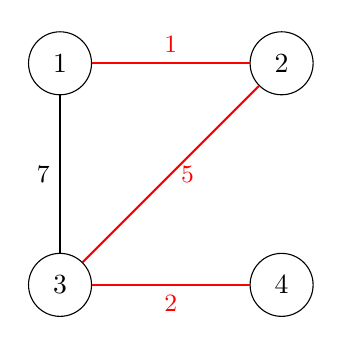
\begin{tikzpicture}[
        vertex/.style={circle, draw, minimum size=8mm},
        edge/.style={draw, thick}
    ]
        % Nodes
        \node[vertex] (1) {1};
        \node[vertex, right=2cm of 1] (2) {2};
        \node[vertex, below=2cm of 1] (3) {3};
        \node[vertex, right=2cm of 3] (4) {4};

        % Edges
        \draw[edge, red] (1) -- (2) node[midway, above] {\small 1};
        \draw[edge] (1) -- (3) node[midway, left]  {\small 7};
        \draw[edge, red] (2) -- (3) node[midway, right] {\small 5};
        \draw[edge, red] (3) -- (4) node[midway, below] {\small 2};
    \end{tikzpicture}
    \caption{Example graph. Red edges form the minimum spanning tree}
    \label{fig:graph-1}
\end{figure}
\FloatBarrier

It arises naturally when dealing with any kinds of networks like constructing efficient electricity grid \cite{bor} or water supply \cite{water}. It is also used in other algorithms -- image registration \cite{image_registration}, handwriting recognition \cite{handwriting} or in the approximate solution for the traveling salesman problem \cite{salesman}.

Algorithms solving the problem and their analysis are presented in many popular resources such as Cormen et al. textbook ``Introduction to Algorithms'' \cite{cormen}, cp-algorithms website \cite{cpalgoPrim} and a comprehensive overview by Eisner \cite{eisner}.

\section{Problem history}
The minimum spanning tree problem has long and rich history going as far back as 1926 when Borůvka used his algorithm to compute the most efficient electricity network for Moravia \cite{bor}. 

The problem was studied for years since and the most widely known contributions were done by Kruskal in 1956 \cite{kruskal} and Prim in 1957 \cite{prim}. These algorithms solve the problem in a greedy manner. The basic argument behind them is that for each vertex its smallest incident edge has to be the part of the minimum spanning tree. Otherwise, such edge would create a cycle with the minimum spanning tree and on this cycle there would be a larger edge also incident to the same vertex, switching these edges in the spanning tree would make its total weight smaller.

That said each algorithm proceeds differently:
\begin{itemize}
    \item \textbf{Borůvka's algorithm}: This algorithm works in phases, in each phase the smallest incident edge to each vertex in the graph is found and these edges are contracted all at once at the end of the phase. Consecutive phases are run until the graph contracts to one vertex. It is proven to work in $O(m\log{n})$ time.
    
    \item \textbf{Kruskal's algorithm}:
    All of the edges are sorted. A disjoint set union is created with each vertex being a different set. Sorted edges are checked in an ascending order when an edge connects two different sets it get contracted and added to the spanning tree under construction. It is proven to work in $O(m\log{n})$ time if the sorting algorithm is comparison based.
    
    \item \textbf{Prim's algorithm}:
    One vertex is picked. Until all vertices are visited the smallest edge joining visited and unvisited vertices is found. It's unvisited end is visited and it's neighboring edges are added to the priority queue on which the unprocessed edges lie. With a standard heap this algorithm runs in $O(m\log{n})$ time and using more complex structures like Fibonacci heap \cite{FredmanTarjan} its complexity decreases to $O(m  + n\log{n})$.
\end{itemize}

Further contributions include Yao \cite{yao} and Cheriton with Tarjan \cite{cherTarj} who independently found different algorithms with $O(m \log{\log{n}})$ complexity. Later Fredman and Tarjan \cite{FredmanTarjan} lowered the complexity to $O(m \beta(m, n))$ where $\beta(m, n)$ is defined as the number of log iterations necessary to map $n$ to number smaller then $\frac{m}n$ and in the worst case for $m = O(n)$ it is $O(m\log^*{n})$. It was shortly after improved to $O(m\log{\beta(m,n)})$ by Gabow et al. \cite{gabowEtAl}. In 2000 Chazelle \cite{C2000} found an algorithm with $O(m\ \alpha(m, n))$ complexity, where the $\alpha$ is the inverse Ackermann function.

The optimal algorithm has been discovered by Pettie and Ramachandrdan in 2002 \cite{optimal}. However the running time complexity of their algorithm is unknown. That said for the practical purposes the problem of finding the mst has been solved for many years as the textbook algorithms have really good complexities and are easy to implement. 

The algorithms presented above all work in a comparison-based model in which the edges are comparable in constant time and no bit manipulation is allowed. If the edge costs are integers and the model allows for bucketing and bit manipulation then the problem is possible to solve in $O(m + n)$ time deterministically, as presented by Fredman and Willard \cite{fredmanWillard}.

It is also possible to verify in linear time that given tree is the minimum spanning tree as shown by Komlós \cite{komlos1984}, King \cite{king1997} and Hagerup \cite{hagerup2009even}.

All of the above algorithms were deterministic, however there also exist randomized algorithms for this problem. Karger, Klein and Tarjan showed in 1995 \cite{kkt} one that runs in $O(m + n)$ expected time. Furthermore in 2005 Chazelle, Rubinfeld and Trevisan \cite{crt} devised a sublinear randomized algorithm which does not find the minimum spanning tree, but rather approximates its total weight.

\begin{table}[H]
\centering
\caption{Minimum spanning tree algorithms. Implemented algorithms highlighted in \textbf{bold}.}
\begin{tabular}{l c c c}
\toprule
\textbf{Name} & \textbf{Year} & \textbf{Complexity} & \textbf{Note} \\
\midrule
Borůvka & 1926 & $O(m\log{n})$ & \\
Kruskal & 1956 & $O(m\log{n})$ & \\
Prim & 1957 & $O(m\log{n})$ & \\
Yao & 1975 & $O(m \log\log(n))$ & \\
Fredman, Tarjan & 1984 & $O(m \beta(m, n))$ & \\
Komlós & 1984 & $O(m + n)$ & verification\\
Galil et al. & 1986 & $O(m \log\beta(m, n))$ & \\ 
Fredman, Willard & 1993 & $O(m + n)$ & bit manipulation \\
Karger, Klein, Tarjan & 1995 & $O(m + n)$ & randomized \\
King & 1997 & $O(m + n)$ & verification \\ 
\textbf{Chazelle} & \textbf{2000} & $O(m\alpha(m,n))$ & \\
Pettie, Ramachandran & 2002 & optimal & unknown complexity\\
\textbf{Chazelle et al.} & \textbf{2005} & sublinear & approximate weight \\
Hagerup & 2009 & $O(m + n)$ & verification \\
\bottomrule
\end{tabular}
\end{table}

\section{Preliminaries}

\subsection{Graphs}
\begin{definition} [Graph \cite{diesel}]
    A graph is a pair $G = (V, E)$ of sets such that $E \subseteq \binom{V}{2}$ and $V \cap E = \emptyset.$
\end{definition}
 Throughout the paper for $G = (V, E)$ we write $V(G)$ to denote $V$ -- the set of vertices (nodes or points) and $E(G)$ to denote $E$ -- the set of edges. 
 
 For any graphs $G$ and $H$ we define the following operations:
\begin{itemize}
  \item $G \cup H = (V', E')$, with $V' = V(G) \cup V(H)$ and $E' = E(G) \cup E(H)$
  \item $G \cap H = (V', E')$, with $V' = V(G) \cap V(H)$ and $E' = E(G) \cap E(H)$
  \item $G \setminus H = (V', E')$, with $V' = V(G) \setminus V(H)$ and $E' = E(G) \setminus E(H)$
\end{itemize}


\begin{definition} [Graph with loops]
 A graph with loops is a pair $G = (V, E)$ of sets such that $E \subseteq V^2$.
\end{definition}

\begin{definition} [Weighted graph]
    Graph $G = (V, E)$ is weighted if there is a function $w : E \xrightarrow{} \mathbb{R_+}$ defined on the edges of $G$. 
\end{definition}
For a given edge $e = \{u, v\}$ we denote its weight (also called cost) $w(e) = w_e = w_{uv}$.

\begin{definition}[Incident \cite{diesel}]
    A vertex $v$ is \textbf{incident} with an edge $e$ if $v\in e$.
\end{definition}
We denote by $E(v)$ set of all edges in $E$ incident with a vertex $v$.

\begin{definition}[Degree \cite{diesel}]
    The degree $d_G(v) = |E(v)|$ of a vertex $v$ is the number of edges incident with $v$.
\end{definition}
Since $G$ is often obvious from the context, we will use the notation $d(v)$ or even $d_v$.

For graphs with loops we define the vertex degree as $d(v) = |E(v)| + |\{v\colon \{v\} \in E\}]$. Loops are counted twice.

\begin{definition}[Average degree \cite{diesel}]
    The number
    \begin{equation*}
        d(G) = \frac1{|V|}\sum\limits_{v \in V}d(v)    
    \end{equation*}
    is the \textbf{average degree} of $G$.
\end{definition}
If it is clear from the context we shorten $d(G)$ to $d$.

Now let us proceed with a few auxiliary lemmas and definitions
\begin{definition}[Subgraph \cite{diesel}]
For graphs $G = (V, E), G' = (V', E')$  If $V' \subseteq V$ and $E' \subseteq E$, then $G'$ is a subgraph of $G$.
\end{definition}
We use the notation $G' \subseteq G$ to denote that $G'$ is a subgraph of $G$.

\begin{definition}[Induced subgraph \cite{diesel}]
    If $G' \subseteq G$ and $G'$ contains all the edges $\{x,y\} \in E$ with $x,y\in V$, then $G'$ is an \textbf{induced subgraph} of $G$. 
\end{definition}
We also say that $V'$ induces $G'$ in $G$.

\begin{definition}[Spanning \cite{diesel}]
    $G' \subseteq G$ is a \textbf{spanning} subgraph of $G$ if $V'$ spans all of $G$, i.e. if $V' = V$.  
\end{definition}

\begin{definition}[Cut of a graph]
    For a given graph $G = (V, E)$ if we have nonempty sets $V_1 \cup V_2 = V$ such that $V_1 \cap V_2 =\emptyset$. We call it a \textbf{cut} and the cut set is the set of edges with one endpoint in $V_1$ and one in $V_2$.
\end{definition}

\begin{definition}[Edge contraction]
    Given a graph $G = (V, E)$ and an edge $uv$ we say that a graph $G' = (V', E')$, where $V' = V(G) \setminus \{u, v\} \cup\{uv\}$ and $E' = \{e \in E: e\in V' \lor (\{w, uv\}\ \text{if}\ wu \in E \lor wv \in E) \}$ has been created through a contraction of edge $uv$.
\end{definition}

\begin{definition}[Graph minor]
    We say that graph $H$ is a minor of graph $G$ if it can be obtained through a sequence of edge contractions beginning with graph $G$.
\end{definition}

\begin{definition}[Path \cite{diesel}]
    A path is a non-empty graph $P = (V,E)$ of the form $V = \{x_0, x_1, ..., x_k\}, E = \{x_0x_1, x_1x_2, ...,x_{k-1}x_k\}$, where $x_i$ are all distinct.   
\end{definition}
The vertices $x_0$ and $x_k$ are \textbf{connected} by $P$ and are called \textbf{ends}.
Throughout the paper we use the notation $P = x_0...x_{k-1}$.

\begin{definition}[Cycle \cite{diesel}]
    If $P = x_0...x_{k-1}$ is a path and $k\geq 3$, then the graph $C := P + x_{k-1}x_0$ is called a \textbf{cycle}.
\end{definition}
Throughout the paper we use the notation $C = x_0...x_{k-1}x_0$.

\begin{definition}[Connected graph \cite{diesel}]
    A graph is called \textbf{connected} if it is non-empty and any two of its vertices are linked by a path in $G$.
\end{definition}

\begin{definition}[Connected component \cite{diesel}]
Let $G = (V, E)$ be a graph. A maximal connected subgraph of $G$ is a \textbf{connected component} of $G$.    
\end{definition}
The components are induced subgraphs and their vertex sets partition $V$.

\begin{definition}[Forest, tree \cite{diesel}]
    An acyclic graph, one not containing any cycles, is called a \textbf{forest}. A connected forest is called a \textbf{tree}.
\end{definition}

\begin{definition}[Leaves, inner vertices \cite{diesel}]
    The vertices of degree 1 in a tree are its \textbf{leaves}, the others are its \textbf{inner vertices}.
\end{definition}

\begin{definition}[Root, rooted tree \cite{diesel}]
    A tree $T$ with one vertex marked as \textbf{root} is called a \textbf{rooted tree}.
\end{definition}

\begin{definition}[Tree cost]
    Cost (also called weight) $w(T)$ of a weighted tree $T$ is the sum of costs of its edges. That is $w(T) = \sum\limits_{e\in E(T)}w_e$.
\end{definition}

\subsection{Minimum spanning tree}
\begin{definition}[Minimum spanning tree]
    Minimum spanning tree of a graph $G$, denoted as $MST(G)$, is a spanning tree with the minimum cost of all of the spanning trees of $G$.
\end{definition}
We will also write $MST$ when the $G$ is known from the context.

\begin{definition}[Minimum spanning tree weight]
For a given graph $G$ let $M(G) = w(MST(G))$ be the weight of its minimum spanning tree.
\end{definition}

\begin{problem}[Minimum spanning tree problem -- optimization]
    For a given graph $G$ find and output the $MST(G)$.
\end{problem}

\begin{problem}[Minimum spanning tree problem -- decision]
    For a given graph $G$ and a number $k$ find a spanning tree $T$ of $G$ such that $w(T) \le k$.
\end{problem}

Following properties assume that the graph $G$ has distinct edge weights:
\begin{theorem} [Strong cut property \cite{eisner}]
\label{cut-property}
For every graph $G$ it holds that $e \in MST(G) \iff e$ is the lightest edge across some cut of $G$.
\end{theorem}
\begin{theorem} [Strong cycle property \cite{eisner}]
\label{cycle-property}
For every graph $G$ it holds that $e \not\in MST(G) \iff e$ is the heaviest edge on some cycle of $G$.
\end{theorem}
Here is the proof of both properties at once due to Eisner \cite{eisner}.
\begin{proof}
    $(\Rightarrow)$ Every $e$ when removed from $MST(G)$ determines a cut across which it is lightest as if there was a lighter edge $e'$ in the cut-set then $MST(G) - e + e'$ would have a smaller weight. Every $e \not\in MST(G)$, when added to the MST(G) creates a cycle on which it is heaviest as if there was a heavier edge $e'$ on the cycle, then once again we would have a contradiction with $MST(G) - e + e'$.

    $(\Leftarrow)$
    We derive contrapositives from the cases just proved. If $e \not\in MST(G)$ then it is a heaviest edge on some cycle and it cannot be the lightest in any cut-set as the cut set would have to intersect the cycle. If $e \in MST(G)$ then it is the lightest in some cut set, so it cannot be the heaviest on any cycle as it would have to have a non empty intersection with the cut-set on which $e$ is the lightest.
\end{proof}

\begin{theorem} [Minimum spanning tree uniqueness]
    If a connected graph $G$ has distinct edge costs then it has exactly one minimum spanning tree.
\end{theorem}
\begin{proof}
Both strong cut property and strong cycle property classify edges into the ones in MST and outside the MST.
\end{proof}

\chapter{Chazelle's \boldmath $O(m\alpha(m,n))$ algorithm}
Chazelle \cite{C2000} proposed in 2000 a new algorithm which solves the minimum spanning tree problem.  He has proven that the algorithm runs in $O(m\alpha(m,n))$ time. It has not been improved on since by any other algorithm with known complexity.

\section{Idea and pseudocode}
The main idea of the algorithm is to partition a graph into smaller subgraphs for which we compute the minimum spanning trees recursively. In order to make it fast the smaller minimum spanning trees together form a spanning tree that is not necessarily minimal. However in the process some edges are proven not to be in the MST and other's have to be reprocessed in a final recursive call.

There are several ideas that work together in this algorithm and this section is devoted to explaining them.

\subsection{Contractible subgraphs}

 It is important to have a certain mindset when considering the MST problem -- that is, one has to think about it in terms of edge contractions. In particular, let us reacall an importanat duality between to properties:
 \begin{itemize}
     \item cut property (\Cref{cut-property}) -- allows us to prove that edge is in the MST and can be contracted.
     \item cycle property (\Cref{cycle-property}) -- allows us to prove that edge is outside of the MST and can be discarded.
 \end{itemize}
These properties are crucial both for the construction of algorithms and for the proofs of certain properties like strong contractibility -- which we will consider now. 

\begin{definition} [Contractible subgraph \cite{C2000}]
A connected induced subgraph $H \subseteq G$ is contractible if and only if $MST(H) \subseteq MST(G)$.
\end{definition}

The notion of contractible subgraphs is helpful when creating divide and conquer algorithms for the MST problem as we shall see below.

Let's say we have a partition of the vertices of a graph $G$ into sets {$V_1, V_2, ..., V_k$} and corresponding induced subgraphs {$G_1, G_2, ..., G_k$}. Denote $G'$ as a graph $G$ after contracting each of the $V_i$ sets of vertices. Now we can see that thanks to the definition of contractible subgraphs we have that
\begin{equation}
MST(G) = \left(\bigcup\limits_{i=1}^{k} MST(V_i)\right) \cup MST(G').
\end{equation}
 
Having that we could recursively apply our MST algorithm and just sum the results.

While contractibility is extremely useful, it is a global property. That is, it depends on the $MST(G)$. Thus proving it from the definition requires computing the $MST(G)$ first.

\begin{definition} [Strongly contractible subgraph]
A connected induced subgraph $H \subseteq G$ is strongly contractible if and only if for all $e,f \in E(G)$ with exactly one endpoint in $H$, there exists path in $H$ which connects $e$ and $f$ and no edge along this path exceeds the cost of both $e$ and $f$.
\end{definition}

\begin{lemma}
If a subgraph $H$of $G$ is strongly contractible then it is contractible.    
\end{lemma}

\begin{proof}
Let's assume $H$ is not contractible, thus $MST(G)\ \cap\ H$ has to have multiple connected components. Let's take a shortest path in $MST(G)$ that connects these components. It is the shortest so it cannot have edges in $H$, let $e, f$ be the first and last edge i.e. the edges which connect $H$ to the $G/H$. 

But the subgraph $H$ is connected and strongly contractible, so there is a path that completes the cycle and lies fully inside $H$ and has all of the edge costs smaller than $\max\{c(e), c(f)\}$. So the largest edge on this cycle lies outside the path in $H$, and by the cycle property it cannot be in the $MST(G)$ -- a contradiction.     
\end{proof}

The notion of strongly contractible subgraphs is local. It allows us to certify contractibility of a given subgraph by looking only at it and its neighborhood.

\subsection{$T$-hierarchy}
\subsubsection{Borůvka}
To introduce the concept of $T$-hierarchy let's first consider Borůvka's algorithm:

\begin{algorithm}[H]
\caption{Borůvka’s Algorithm}
\label{bor}
\begin{algorithmic}[1]
\Function{Boruvka}{$G \colon \texttt{Graph}$}
    \State $F \gets \emptyset$ 
    \While{$|E| > 0$}
        \State $F \gets F\ \cup\ $ \Call{Boruvka-step}{$G$}
    \EndWhile
    \State \Return $F$
\EndFunction
\end{algorithmic}
\end{algorithm}

\begin{algorithm}[H]
\caption{\textsc{Boruvka-step}}
\label{bor-step}
\begin{algorithmic}[1]
\Function{Boruvka-step}{$G\colon \texttt{Graph}$}
    \State $F \gets \emptyset$
    \State $marked \gets \emptyset$
    \For{$v \in V(G)$}
        \State $e \gets \arg\min{\{c(e)\colon e \in E(v)\}}$
        \State $marked \gets marked \cup \{e\}$
    \EndFor
    \For{$e \in marked$}
        \State \Call{contract}{$G, e$}
        \State $F$\Call{.insert}{$e$}
    \EndFor
    \State \Return $F$
\EndFunction
\end{algorithmic}
\end{algorithm}
\FloatBarrier
Let's consider what happens to a connected graph $G$ during the \Cref{bor-step}. Let $n, m$ be number of vertices and edges in $G$. We can see that the number of vertices in the resultant graph will be at most $\frac{n}{2}$, i.e. it drops by a factor of $2$. So the \Cref{bor} calls \Cref{bor-step} only $O(\log{n})$ times. 

 Unfortunately the number of edges $m$ doesn't always drop by a multiplicative factor. In the worst case only $\frac{n}{2}$ edges will be contracted. Given the fact that \textsc{Boruvka-step} can be performed in $O(n + m)$ time gives the total running time $O(m\log{n})$. 
 
 Consider what would happen if the number of edges decreased in every iteration by a multiplicative factor $q$, then the whole algorithm would run in time \begin{equation*}
     \left(n + m\right) + \left(\frac{n}{2} + qm\right) + \left(\frac{n}{4} + q^2m\right) ... \leq 2n + \frac{1}{1-q} m = O(n + m).
 \end{equation*}

So if we found a way to remove a factor of edges in linear or almost linear time, then we could also perform a single \Cref{bor-step} in linear time to also decrease the number of vertices by some factor and have a routine that works in linear or slightly larger time.

\subsubsection{Borůvka hierarchy}
Consider the sequence of graphs produced during consecutive \textsc{Boruvka-step} invocations. Each consecutive graph is a minor of the previous one, as \textsc{Boruvka-step} only performs edge contractions. Being a minor is a transitive property so a graph obtained after any number of \Cref{bor-step} will be a minor of every previous one.

Now looking at just one \Cref{bor-step} we can also think about it as of identifying multiple vertices as one, in this spirit we could create a forest which has two sets of vertices -- first set corresponds to vertices in original graph and the second one has vertices from the resultant minor. We can connect vertices $v$ from the first set and $w$ from the second set if $w$ was created by contracting $v$ and some other vertices. See \Cref{fig-mst} and \Cref{fig-forest}.

\begin{figure}[ht!]
    \centering
    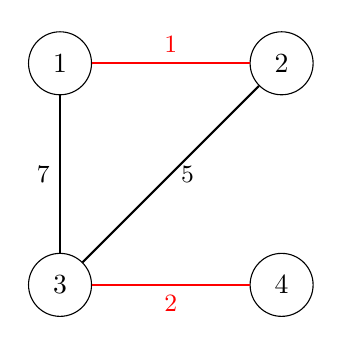
\begin{tikzpicture}[
        vertex/.style={circle, draw, minimum size=8mm},
        edge/.style={draw, thick}
    ]
        % Nodes
        \node[vertex] (1) {1};
        \node[vertex, right=2cm of 1] (2) {2};
        \node[vertex, below=2cm of 1] (3) {3};
        \node[vertex, right=2cm of 3] (4) {4};

        % Edges
        \draw[edge, red] (1) -- (2) node[midway, above] {\small 1};
        \draw[edge] (1) -- (3) node[midway, left]  {\small 7};
        \draw[edge] (2) -- (3) node[midway, right] {\small 5};
        \draw[edge, red] (3) -- (4) node[midway, below] {\small 2};
    \end{tikzpicture}
    \caption{Example graph. Red edges are contracted in the first run of \Cref{bor-step}.}
    \label{fig-mst}
\end{figure}

\begin{figure}[ht!]
    \centering
    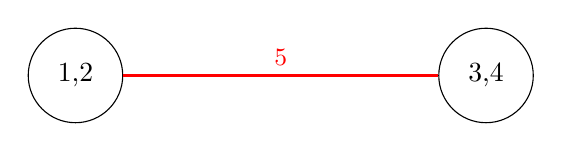
\begin{tikzpicture}[
        vertex/.style={circle, draw, minimum size=12mm},
        edge/.style={draw, thick}
    ]
        % Super-nodes
        \node[vertex] (A) {1,2};
        \node[vertex, right=4cm of A] (B) {3,4};

        % Edge
        \draw[edge, red] (A) -- (B) node[midway, above] {\small 5};
    \end{tikzpicture}
    \caption{The example graph minor after the \Cref{bor-step} -- also the $C_{1,2,3,4}$ graph.}
\end{figure}

\begin{figure}[ht!]
\centering
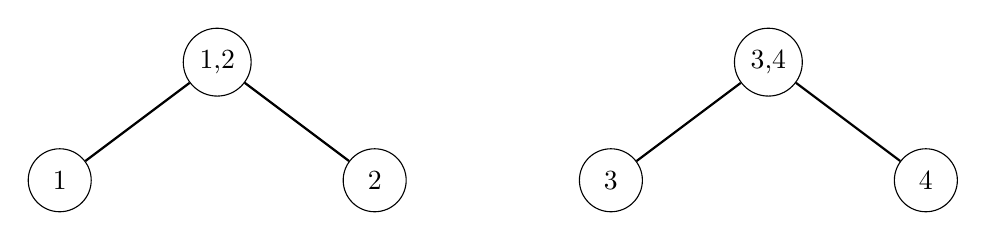
\begin{tikzpicture}[
    level distance=1.5cm,
    every node/.style={circle, draw, minimum size=8mm},
    edge from parent/.style={draw, thick}
]
% First tree
\node {1,2}
    child[sibling distance=4cm] { node {1} }
    child[sibling distance=4cm] { node {2} };

% Second tree (shifted to the right)
\node at (7,0) {3,4}
    child[sibling distance=4cm] { node {3} }
    child[sibling distance=4cm] { node {4} };
\end{tikzpicture}
\caption{Forest corresponding to a single iteration of \Cref{bor-step}.}
\label{fig-forest}
\end{figure}



If we extend that forest by adding sets of vertices corresponding to minor's in each consecutive \Cref{bor-step} iteration we will get a tree $T$, which root represents a contraction of all vertices into a single node. Each layer below it corresponds to the minor from the previous iteration, and leafs of this tree $T$ are just the vertices of the original graph $G$ for which we want to find the minimum spanning tree. See \Cref{t-h} below.

\begin{figure}[H]
\centering
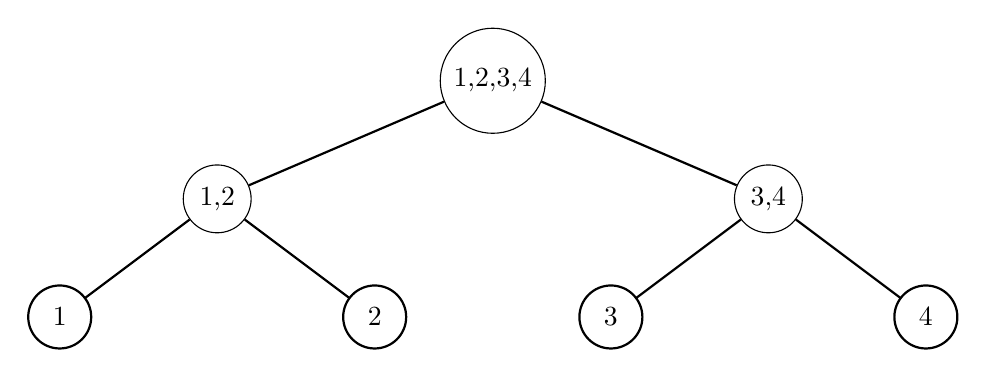
\begin{tikzpicture}[
    level distance=1.5cm,
    every node/.style={circle, draw, minimum size=8mm},
    edge from parent/.style={draw, thick}
]
    % Root
    \node {1,2,3,4}
        child[sibling distance=7cm] { node {1,2}
            child[sibling distance=4cm] { node {1} }
            child[sibling distance=4cm] { node {2} }
        }
        child[sibling distance=7cm] { node {3,4}
            child[sibling distance=4cm] { node {3} }
            child[sibling distance=4cm] { node {4} }
        };
\end{tikzpicture}
\caption{$T$-hierarchy constructed by the \Cref{bor}.}
\label{t-h}
\end{figure}

\begin{figure}[H]
    \centering
    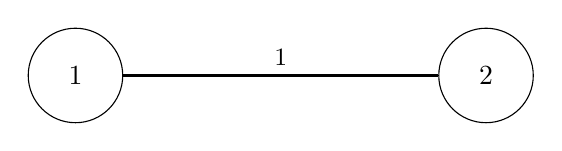
\begin{tikzpicture}[
        vertex/.style={circle, draw, minimum size=12mm},
        edge/.style={draw, thick}
    ]
        % Super-nodes
        \node[vertex] (A) {1};
        \node[vertex, right=4cm of A] (B) {2};

        % Edge
        \draw[edge] (A) -- (B) node[midway, above] {\small 1};
    \end{tikzpicture}
    \caption{The $C_{1,2}$ graph}
\end{figure}
\FloatBarrier

\begin{definition}[$T$-hierarchy]
    $T$-hierarchy is a rooted tree $T$, whose leaves correspond to the vertices of a given graph $G$ and the internal nodes represent contractions of all of the leaves below them.  
\end{definition}
In particular root corresponds to the contraction of the whole graph $G$ and a subtree of $T$ corresponds to a minor of the graph $G$.

\begin{definition}[$z_i \texttt{ and } C_{z_i}$]
We introduce the notation that $z_i$ is an internal node of the tree $T$ and $C_{z_i}$ is a graph whose vertices are the children of $z_i$. The edge between vertices $u$ and $v$ in this graph corresponds to the smallest edge (if it exists) joining sets of vertices of $G$ -- the leaves below $u$ and $v$ in the $T$-hierarchy respectively.   
\end{definition}

Now the $T$-hierarchy constructed by the Borůvka's algorithm has an important property. If you look at any node in the hierarchy its correspondent set of vertices of $G$ induces a contractible subgraph in $G$. This property follows directly from the fact that the hierarchy was created by contracting the edges which belong to the $MST(G)$.

If we were given a $T$-hierarchy with this property, we could compute the minimum spanning tree using the divide and conquer method with the following lemma:
\begin{lemma}[$MST$ construction using $T$-hierarchy]
Given a graph $G$ and corresponding $T$-hierarchy such that for every $z\in V(T)$ its $C_{z}$ is contractible we can find the $MST(G)$ using the following identity:
\begin{equation*}
    MST(G) = \bigcup\limits_{z\in T}MST(C_z).
\end{equation*}
\label{divide-conq}
\end{lemma}
\begin{proof}
    We repeatedly apply (2.1) until the $G'$ is fully contracted. Consider what happens after one application of (2.1) to the original graph $G$ and a partition into the contractible subgraphs defined by the bottom layer of $T$ ($z$ such that all of $z$'s children are leaves). 
    
    For example for \Cref{t-h}, after the first application of (2.1) we are left with a $G'$ and its $T$-hierarchy $T'$ which was obtained from $T$ by pruning all of the leaves $1, 2, 3$ and $4$. 
\end{proof}

\subsection{Reverse the construction schedule}
One of the main ideas behind the algorithm is to reverse the MST construction schedule. First we could create a hierarchy $T$ such that each layer represents a partition of the graph $G$ into contractible subgraphs. Then we would calculate the $MST(G)$ recursively using the \Cref{divide-conq}.

\subsubsection{Corruption}
Nevertheless, calculating the $T$-hierarchy proves to be a difficult task. To make this step fast Chazelle decided to loosen the requirements put on the $T$-hierarchy. During its creation some edges will become corrupted, that is their weight will be purposefully made higher then original. The resultant $T$-hierarchy will have its internal nodes contractible, but in terms of the \textbf{working cost} of the edges and not counting the \textbf{discarded} edges (both notions will be defined later). 

It is important to mention that all of the \textbf{discarded} edges and also the edges for which the \textbf{working cost} is different than their original cost will be reprocessed later with their costs reverted back to the original.

\begin{remark}[Edge corruption]
    Each edge of the graph $G$ has its original cost and current cost associated with it. The current cost can change during a construction of $T$, but will never be lower than the original cost. We call edges \textbf{corrupted} when their current and original costs differ.

    %When referring to the current cost of an edge, unless explicitly stated otherwise, we refer to the current cost at the moment when the $T$ has been constructed and the costs are now frozen.%
\end{remark}

\subsubsection{Prim}
In order to understand why and how the corruption happens and what are the working costs of the edges referred to in the previous subsection we need to first understand how the $T$-hierarchy is built. 

Let's first consider Prim's algorithm as it will be the basis for the $T$-hierarchy construction. We can think about it as picking a vertex $v$ and sequentially contracting entire graph to it edge by edge. It also can be thought of as a Dijkstra analogue: there are visited and unvisited nodes and we always visit the closest one, but not the closest one to the origin $v$ like in Dijkstra.

\begin{algorithm}[H]
\caption{Prim's Algorithm}
\begin{algorithmic}[1]
\Function{Prim}{$G\colon \texttt{Graph}$}
    \State $v \gets$ \Call{pick-any-vertex}{$G$}
    \State $F \gets \emptyset$
    \While{$E(G) \neq \emptyset$}
        \State $e \gets$ \Call{smallest-edge-adjacent-to}{$v$}
        \State \Call{contract-edge}{$e, G$}  \Comment{Contracts other vertex $u$ into $v$}
        \State $F \gets F \cup \{e\}$
    \EndWhile
    \State \Return $F$
\EndFunction
\end{algorithmic}
\end{algorithm}
\FloatBarrier

\subsubsection{Building the $T$-hierarchy}
The Prim's algorithm does not care about the already visited vertices: when a vertex $v$ is processed its edges are pushed on a priority queue and the vertex can be forgotten of.

To build the $T$-hierarchy we will perform a Prim's algorithm but with two important modifications:
\begin{itemize}
    \item we maintain a structure on the visited vertices -- this structure is the $T$-hierarchy being built.
    \item as a priority queue we will use soft heaps, a heap-like data structure devised by Chazelle.
\end{itemize}

The exact construction schedule and soft heaps will be discussed thoroughly later. For the purpose of this introduction let us mention their most important properties:

\begin{itemize}
    \item Soft heaps are responsible for the edge corruption.
    \item $T$-hierarchy is created \textbf{bottom-up} -- when a $C_z$ is assembled all of its children are constructed too and the current costs of edges inside them are frozen. When the $C_z$ has been constructed it gets contracted to a vertex and put inside its parent.
    \item In the process of construction some edges are \textbf{discarded} -- these edges were necessarily bad.
\end{itemize}

Let us finally introduce the crucial auxiliary notions for this algorithm:
\begin{definition}[Border edge]
    During the Prim's algorithm if the edge joins a visited and an unvisited node, then its a \textbf{border edge}.
\end{definition}

In the Chazelle's algorithm context during the construction of $T$-hierarchy we maintain a structure on visited nodes, that is, the $C_z$ graphs. We use the same name border edge for the edges joining visited and unvisited vertices. We also say that a border edge $\{u, v\}$ joins a $C_z$ to an unvisited vertex $v$ when the visited vertex $u$ is under the $z$ node in the $T$-hierarchy.

\begin{definition}[Bad edge]
    A border edge $e$ becomes bad if it is corrupted and has one endpoint in a current $C_z$ in the moment of its contraction.
\end{definition}
    We will sometimes reset the current costs of the edges, but once the edge becomes bad it always remains bad, even after the reset.


\begin{definition}[Working cost]
    Working cost of an edge $e$ is its current cost if it is bad, otherwise it is its original cost.
\end{definition}

\subsubsection{Soft heap}
Soft heap is a minimum heap devised by Chazelle, which is a workhorse for the algorithm. It breaks the traditional $O(\log{n})$ bound for heaps for all of its operations, but at the cost of corruption: some elements may have their keys increased. 

Each element inserted into the soft heaps has its original key, and also a ckey - they are equal in the beginning. The soft heap maintains an ordering using the ckeys and ckeys cannot be lower then keys. 

Soft heap allows for \texttt{make-heap}, \texttt{insert}, \texttt{meld}, \texttt{pop-min} and \texttt{delete} operations. Each of them runs in $O(1)$ amortized time, but for the \texttt{insert} operation which runs in $O(\log{\frac{1}{\epsilon}})$ amortized time. The $\epsilon$ parameter is set in the \texttt{make-heap}. 

Soft heap maintains an invariant that there are at most $\epsilon n$ corrupted elements on the heap, where $n$ is the number of inserted elements -- not to confuse with the number of elements currently stored in the heap.

\subsection{Pseudocodes}
\begin{algorithm}
\caption{Recursive MST Algorithm}
\begin{algorithmic}[1]
\Function{mst}{$G \colon \texttt{Graph}, \ t \colon \texttt{int}$}
    \If{$t = 1 \ \lor\ n = O(1)$} 
        \State \Return \Call{Boruvka}{$G$} \Comment{STEP 1}
    \EndIf
    \State $G_0, F_0 \gets$ \Call{Boruvka-steps}{$G, c$} \Comment{STEP 2}
    \State $T, B \gets$ \Call{construct-$T$-hierarchy}{$G_0$} \Comment{STEP 3}
    \State $F \gets \bigcup_{C_z \in T} \Call{mst}{C_z / B, \ t-1}$ \Comment{STEP 4}
    \State \Return $F_0 + \Call{mst}{F + B, \ t}$ \Comment{STEP 5}
\EndFunction
\end{algorithmic}
\label{cmst}
\end{algorithm}

\Cref{cmst} presents a basic pseudocode for the whole algorithm. It takes a graph $G$ and a number $t$ as inputs and returns $MST(G)$. The parameter $t$ is used in creation of $T$-hierarchy for tuning the recursion so that we have the double induction necessary for the complexity bound involving the inverse Ackermann function.
\begin{itemize}
    \item \textbf{STEP 1} This is the base case:  we just run the \Cref{bor} if the graph is small enough or $t = 1$. As the algorithm is recursive we need a base case.
    \item \textbf{STEP 2} We apply $c$ consecutive \textsc{Boruvka-step}s to the graph $G$ and return the resultant minor $G_0$ and the forest of contracted edges $F_0$.
    \item \textbf{STEP 3} This step is the hardest and contains most of the actual algorithm. Pseudocode and its analysis is provided below.
    \item \textbf{STEP 4} We recursively call \Cref{cmst} on $C_z$'s of all the internal nodes of $T$-hierarchy with bad edges removed from them. We collect the returned trees into a forest $F$.
    \item \textbf{STEP 5} We recursively call \Cref{cmst} on a graph created from bad edges $B$ and forest $F$ as we need to reprocess the bad edges. 
\end{itemize}

Let's get back to the most important part: the construction of $T$-hierarchy. Here is the pseudocode:
\begin{algorithm}[H]
\caption{$T$-hierarchy construction}
\begin{algorithmic}[1]
\Function{construct-$T$-hierarchy}{$G_0 \colon \texttt{Graph}$}
    \State \texttt{Cz} $\gets \emptyset$
    \State \texttt{H} $\gets \emptyset$ \Comment{set of soft heaps}
    \State \texttt{B} $\gets \emptyset$ \Comment{set of bad edges}
    \State \texttt{min-links} $\gets \emptyset$
    \State \Call{pick-starting-vertex}{}
    \While{ \Call{edges-on-heaps}{}}
        \If{\Call{met-desired-size}{}}
            \State \Call{retraction}{}
        \Else
            \State $e \gets$ \texttt{H}.\Call{pop-min}{}
            \If{\Call{need-fusion}{}}
                \State \Call{fusion}{}
            \EndIf
            \State \Call{extension}{}
        \EndIf
    \EndWhile
    \While{ \texttt{Cz}.\Call{length}{} > 1}
        \State \Call{retraction}{}
    \EndWhile
    \State \Return \texttt{Cz[1]}, \texttt{B}
\EndFunction
\end{algorithmic}
\label{tconstr}
\end{algorithm}

\begin{remark}
    All of the functions in the pseudocode above have the access to the state variables defined at the beginning. Thus, they were omitted from the function calls as they would clutter the pseudocode.
\end{remark}

As stated previously, the $T$-hierarchy construction mimics the Prim's algorithm: in each iteration of the loop we pop the smallest edge from the heaps and process it. 

Let's first consider the desired properties of $T$:
\begin{itemize}
    \item each $C_z$ has to be strongly contractible in terms of working costs and ignoring discarded edges,
    \item each $C_z$ has a desired size which it should attain before being contracted -- however, the exact sizing is only important for the runtime complexity analysis and will be discussed there.
\end{itemize}

Let's consider the variables used in \Cref{tconstr}.
\begin{itemize}
    \item \texttt{Cz} -- Is a stack of graphs which represent $C_z$'s \textbf{under construction} -- the so called active path. At the bottom of the stack lies the $C_{z_{root}}$ which corresponds to the root of $T$. Each consecutive stack item corresponds to the chld in $T$ of the previous one.   
    We use the notation $C_{z_1}, C_{z_2} ...C_{z_k}$ to enumerate all of the $C_z$ under construction.
    \item \texttt{H} is a minimum heap containing all of the border edges. For the complexity reasons (discussed later) it has to be a 2-dimensional array of soft heaps: if the active path is $C_{z_1}, C_{z_2} ...C_{z_k}$ then we have a $\texttt{H[i][j]} \text{ for all } i,j \in \{0, 1,..., k\}, i \leq j$.
    \item \texttt{B} -- a graph of the bad edges.
\end{itemize}

In order not to produce to many bad edges and enforce contractibility of the $C_z$'s following invariants will be maintained during the construction of the $T$-hierarchy.

\begin{invariant}[\cite{C2000}]
We keep an edge called a chain-link joining $C_{z_i}$ and $C_{z_{i+1}}$ for all $i \in \{1, 2, ..., k - 1\}$. Its current cost is:
\begin{enumerate}
    \item[(i)] at most that of any border edge incident to $C_{z_1} \cup \dots \cup C_{z_i}$
    \item[(ii)] less than the working cost of any edge joining 2 distinct $C_{z_j}$ with $j \leq i$
\end{enumerate}
\label{i1}
\end{invariant} 
To enforce the latter condition efficiently we maintain a min-link (if it exists) for each pair $i < j$ -- an edge of minimum working cost joining $C_{z_i}$ and $C_{z_j}$.

\begin{invariant}[\cite{C2000}]
For all $j$, the border edges $\{u, v\}$ with $u \in C_{z_j}$, the edges are stored in a soft heap -- denoted either \texttt{H[j][j]} or in one \texttt{H[i][j]}, where $0 \leq i < j$. No edge appears in more than one soft heap.

Membership in \texttt{H[j][j]} implies that $v$ is incident to at least one edge stored in some \texttt{H[i][j]}.

Membership in \texttt{H[i][j]} implies that v is also adjacent to $C_{z_i}$ but not to any $C_{z_l}$ in between ($i < l < j$). It is extended to \texttt{H[0][j]} and it means that $v$ is not incident to any $C_{z_l}$ with $(l < j)$.
\label{i2}
\end{invariant}

As shown in the pseudocode the construction of $T$-hierarchy works in a loop with three main operations: \textsc{retraction}, \textsc{fusion} and \textsc{extension}.
\subsubsection{\textsc{retraction}}
When the $C_{z_k}$ has attained its desired size we contract it to $1$ vertex and add this vertex to its parent -- $C_{z_{k-1}}$. We need to maintain a valid state for:
\begin{itemize}
    \item \texttt{H} -- we meld \texttt{H[k][*]} to appropriate \texttt{H[k-1][*]} -- implied by Invariant 2. \texttt{H[k-1][k]} and \texttt{H[k][k]} have to be destroyed and each edge has to be examined again -- that's were the corrupted edges (bad now) are \textbf{discarded}. Some edges will now have the same origin -- only the smallest one of them is retained in a heap implied by Invariant 2.
    \item \texttt{min-links} -- we have to pop \texttt{min-links[k]} and update \texttt{min-links[k-1]} using it.
    \item \texttt{Cz[k-1]} edges -- we need to update the edges to the newly added vertex. 
\end{itemize}

\subsubsection{\textsc{fusion}}
We have a border edge $e$ (called \textbf{extension edge}) that we want to use for the extension but doing so would violate the Invariant 1. Out of all pairs $i,j$ we need to find one with the lowest $i$ that \texttt{min-links[i][j]} working cost is smaller or equal to the current cost of $e$. Let's say we found the edge $e = \{a,b\}$ for some $a \in C_{z_i}, b\in C_{z_j}$. 

We contract all of the edges with both endpoints in $\{a\} \cup C_{z_{i+1}}\cup ... \cup C_{z_k}$ into $a$ and now the edge $e$ has one of its endpoints in $a$. Maintaining valid state for \texttt{min-links} and \texttt{H} is analogous to the one in retraction, but now we do multi-pops instead of normal pops. That said this operation is not a retraction -- no new vertex is created and added to $C_{z_i}$.

\begin{remark}
    The edges contracted during the fusion have to be somehow returned from the \textsc{construct-$T$-hierarchy} function and added to the $F$ accumulator. It can be done explicitly or they can be stored inside $a$ and added during the construction of $MST(a)$ in \textbf{STEP 4}. 
\end{remark}

\subsubsection{\textsc{extension}}
 We are given an extension edge $e$ which connects the end of the active path $C_{z_k}$ (guaranteed by the earlier fusion) to an unvisited vertex $v$. We need to:
\begin{itemize}
    \item process all of the edges of $v$ -- old border edges need to be removed from the heaps and used to update min-links. New border edges have to be pushed onto the heaps implied by \Cref{i2}.
    \item push $v$ onto the \texttt{Cz}.
\end{itemize}

That's an in-depth overview of what happens during the construction of $T$-hierarchy. It is similar to the Prim's algorithm -- we process edges until there are no more edges left (i.e. we have processed the whole graph). If the lowest node has met its desired size we perform retraction and otherwise we find the minimum border edge among all of the heaps and perform the extension (along with fusion if necessary).

\section{Correctness}
Let's first consider the invariants which are maintained in the \textbf{STEP 3}.
\begin{lemma}
    During the \textbf{STEP 3} Invariants 1 and 2 are maintained.
\end{lemma}
\begin{proof}
Consider \Cref{i1} -- retraction obviously maintains it as it only removes the last chain-link and only changes the now last $C_z$, so it won't introduce problems neither with (i) nor with (ii). For the extension remember that we first call fusion if the (ii) cannot be enforced with a given border edge. The sole purpose of fusion is to maintain (ii) invariant. After the fusion we will have that the extension edge can become a new chain link as thanks to the fusion it satisfies (ii).

\Cref{i2} is self explanatory -- it gives us the recipe of how to store the border edges and we follow it.
\end{proof}

These invariant make sure that if we maintain them then we will produce contractible $C_z$'s which is important as it allows us to use divide and conquer in \textbf{STEP 4}.

To prove this we will use the notion of strong contractibility, the fact that it can certify contractibility of a subgraph by only looking at it and its incident edges is paramount. We want to prove the following lemma:

\begin{lemma}[Lemma 3.2 in \cite{C2000}]
\label{sc}
With respect to working costs and excluding discarded edges, $C_z$ is strongly contractible at the time of its contraction (during retraction), and the same holds for every fusion edge $(a, b)$.
\end{lemma}

\begin{proof}    
Consider the fact that $C_z$ grows monotonically, since  retractions add one vertex to it and fusions may add new neighboring edges to it. As only border edges can be discarded, therefore $C_z$ will also not loose any edges inside it. So we only need to consider the moment right before the retraction.

Let's only consider the case when no fusion occurred, consider any two edges $e, f$ which are incident to $C_z$ right before the retraction. As no fusion ever happened the $C_z$ was created solely by retracting chain links, thus it has a spanning tree made out of only chain-links.  Now we can find the path $\pi$ between e and f that is entirely inside this spanning tree. Consider the edge $g$ with the largest current cost (in time of its selection as chain link) in case of ties pick one that was selected for extension last. Now let's say that $g = (u,v)$ where at time of the extension $u$ was inside $C_z$ and $v$ was not. Without loss of the generality $u$ is between $e$ and $v$ on the path $\pi$. Now if $e$ is not a border edge than it has to link to a $C_z$ earlier on the active path, so by the \Cref{i1}(ii) it has to have its working cost larger than $g$. In the case it is a border edge, if it had a smaller working cost, then we would have picked it before $g$ for the extension edge.
\end{proof}

For the correctness proof we will need a following lemma:
\begin{lemma}[Lemma 3.1 in \cite{C2000}]
\label{bad}
If the edge of $G_{0}$ is not bad and it lies outside of $F$, then it lies outside of $MST(G_0)$
\end{lemma}
The proof of this lemma relies heavily on the \Cref{sc}.

\begin{theorem}[Correctness proof]
    The \Cref{cmst} when given a connected graph $G$ as an input returns the $MST(G)$. 
\end{theorem}
\begin{proof}
The proof is an induction on $t$ and $n$.

For the base case -- small $n$ or $t=1$ -- the algorithm runs just the \textbf{STEP 1} e.g. runs the \textsc{boruvka} algorithm on the given graph which is proven to work.

Now consider the inductive step with sufficiently large $t$ and $n$ (so that we do not fall into \textbf{STEP 1}). First let $G_0$ and $F_0$ denote respectively a minor of $G$ which is the result of \textbf{STEP 2} and the forest of contracted edges during \textbf{STEP 2}. By the correctness of the \textsc{boruvka} and the \textsc{boruvka-steps} algorithms we know that $F_0 \subseteq MSF(G)$ and $MSF(G_{0}) \cup F_{0} = MSF(G)$. As the whole function returns \textsc{mst}($F \cup B, t$) we need to prove that $MST(F \cup B) = MST(G_{0})$ which is directly implied by \Cref{bad}. 
\end{proof}

\section{Running time complexity}

Let us first define few functions for bounding the complexity.
\begin{definition}[Ackermann function]    
For all $i, j \in \mathbb{N}$ let Ackermann function $A$ be defined as:
\begin{align*}
    A(i, j) = 
    \begin{cases}
        2j & \text{if $i = 0$,} \\
        0 & \text{if $j = 0$,} \\
        2 & \text{if $j = 1$,} \\
         A(i - 1, A(i, j -1)) & \text{otherwise.}
    \end{cases}
\end{align*}
\end{definition}

\begin{definition}[Inverse Ackermann function]
    Define inverse Ackermann function as $\alpha(m, n) = \min{\{ i \geq 1\colon A(i, 4\lceil\frac{m}n\rceil) > \log{n}\}}$
\end{definition}
\begin{definition}[S function]
For all $i, j \in \mathbb{N}$ let function $S$ be defined as:
\begin{align*}
    S(i, j) = 
    \begin{cases}
        2j & \text{if $i = 1$,} \\
        2 & \text{if $j = 1$,} \\
        S(i, j - 1) S(i-1, S(i, j-1)) & \text{otherwise.}
    \end{cases}
\end{align*}
\end{definition}

As the algorithm is recursive the complexity proof will be inductive. To bound the running time of each step of the algorithm following lemmas will be used.

\begin{lemma}[Decay lemma, Lemma 4.1. in \cite{C2000}]
The total number of bad edges produced while building T is $|B| \leq \frac{m_0}2 + d^3n_0$.
\label{decay}
\end{lemma}
\begin{lemma}[Lemma 4.2. in \cite{C2000}]
\label{inserts}
Total number of inserts in all the heaps is at most $4m_0$.
\end{lemma}

The proof of the lemma above is based on \Cref{i2} and uses amortized analysis.

\begin{theorem}[Lemma 5.1. in \cite{C2000}]
If $d=c\lceil(\frac{m}n)^\frac13\rceil$ and $t = \min\{i > 0\colon n \leq S(i, d)^3\}$, then $t = O(\alpha(m, n))$
\label{acker}
\end{theorem}

The theorem below along with \Cref{s4,s5} are proven by one induction and they reference each other in the induction step. 
\begin{theorem}
    There exists a constant $b$ that for any graph $G$ and positive integer $t$ such that \textsc{mst}$(G, t)$ runs in time $bt(m + d^3(n-1))$. Here $d$ is an integer large enough so that $n \leq S(t, d)^3$.
\label{ctime}
\end{theorem}
\begin{lemma}[Bound on \textbf{STEP 2} and \textbf{STEP 3}]
    There exists a constant $b$ such that for any graph $G$ and positive integer $t$ \textbf{STEP 2} and \textbf{STEP 3} take at most $\frac{b}2(n+m+d^2n_0)$ time. 
    \label{s23}
\end{lemma}

\begin{proof}
    \textbf{STEP 2} takes $O(n + m)$ time we can hide it in the $b$ constant and we are left with the \textbf{STEP 3}.

    The construction of the $T$-hierarchy is dominated by the soft heap operations and changes to \texttt{min-links}. Let's first consider the soft heap operations:
    \begin{itemize}
        \item \texttt{insert}s -- From \Cref{inserts} we know that these operations take $O(m_0) = O(m)$ time.
        \item \texttt{make-heap}s -- These operations only happen at the start and during the extension, which happens exactly $n_0 - 1$ times (Consider Prim's algorithm). Depth of the $T$-hierarchy is $d$ thus in the worst case we could create $d$ new heaps during $1$ extension. It follows that there are at most $O(dn_0)$ of them
        \item \texttt{meld}s -- There cannot be more melds than \texttt{make-heaps}, thus there is at most $O(dn_0)$ of them.
        \item \texttt{pop-min}s -- There are exactly $n_0 - 1$ of them.
    \end{itemize}

    Now for the \texttt{min-links} operations we can see that there are always less then $d^2$ elements in \texttt{min-links} array. And all updates and checks during the extension, fusion and retraction can be done in linear time of the size of the array. Thus there are $O(d^2n_0)$ operations on \texttt{min-links}.

    Summing these values up and picking a sufficiently large $b$ we get the $\frac{b}2(n+m+d^2n_0)$ bound.
\end{proof}

\begin{lemma}[Bound on \textbf{STEP 4}]
    There exists a constant $b$ such that for any graph $G$ and positive integer $t$ \textbf{STEP 4} takes at most $b(t-1)(m_0 - |B| + dn_0)$ time.
    \label{s4}
\end{lemma}
The proof follows from the induction.

\begin{lemma}[Bound on \textbf{STEP 5}]
    There exists a constant $b$ such that for any graph $G$ and positive integer $t$ \textbf{STEP 5} takes at most $bt(n_0 - 1 + |B| + d^3(n_0 - 1)$) time.
    \label{s5}
\end{lemma}
The proof follows from the induction.

\begin{proof}[Proof of \Cref{ctime}]

The proof is by induction on $t$ and $n$.

\textbf{Base case}:
for $n$ and $t$ small enough we only call \textbf{STEP 1} i.e. compute the $MST(G)$ in constant time as the $n$ and $t$ are less than some constant. We need to pick $b$ large enough so that the theorem holds.

\textbf{Induction step}:
Fix $n$ and $t$ and consider a graph $G$ with $n$ vertices. From \Cref{s23,s4,s5} we get the bound for each step of the algorithm. We can now finish the proof by summing them up:
\begin{align*}
\frac{b}2\left(n+m+d^2n_0\right) & + b(t-1)\left(m_0 - |B| + dn_0\right) + bt\left(n_0 - 1 + |B| + d^3(n_0 - 1)\right) \\
 & \leq btm_0 + b\left(\frac{m}2 - m_0 + |B|\right) + 2btd^3n_0 + \frac{bn}2 \\
 & \leq btm - b(m - m_0)\left(t - \frac12\right) + 3btd^3n_0 + \frac{bn}{2}.
\end{align*}
The last inequality follows from \Cref{decay}.

Now remember that $n_0 \leq \frac{n}{2^c}$ because we performed $c$ times \textsc{boruvka-steps} at the beginning. Moreover, even after a single \textsc{boruvka-step} we get $m - m_0 > \frac{n}{2}$ and since we are in the inductive case $t > 1$ holds. Using these inequalities we can finally show that it is bounded by $bt\left(m+ d^3(n-1)\right)$.
\end{proof}

\begin{theorem}
    The MST of a connected graph with n vertices and m edges can be computed in $O(m\alpha(m, n))$ time.
\end{theorem}
\begin{proof}
    It follows directly from \Cref{ctime,acker}.
\end{proof}


\chapter {Chazelle-Rubinfeld-Trevisan sublinear weight finding algorithm}
The problem of finding the minimum spanning tree for a given graph requires at least linear time in terms of edges and vertices. However there might be a case in which only the weight of the MST is needed. This still would require linear time for a deterministic algorithm as each edge potentially can be in the MST, but it opens a possibility for faster approximate algorithms. 

\begin{problem}[Minimum spanning tree weight approximation]
    Given a graph $G$ and parameter $\epsilon$ return an approximation $M^*(G)$ of the $M(G)$ such that $\mathbb{P}(|M^*(G) - M(G)| \leq \epsilon M(G)) \geq \frac34$.
\label{mstapprox}
\end{problem}

Chazelle, Rubinfeld and Trevisan devised an algorithm that solves this problem \cite{crt}. To achieve this result they put additional constraint on the input graph -- all edge weights have to be in the set $\{1, 2,\dots, w\}$. Their algorithm's expected running time is $O(dw\epsilon^{-2}\log{\frac{dw}\epsilon})$ so it depends on $\epsilon$ and the average degree $d$ of the input graph. Clearly e.g. for constant $\epsilon$ and constant upper bound $w$ on edge weights the algorithm runs in time $O(d\log{d})$ which is sublinear for sparse graphs.

\section{Definitions}
\begin{definition}
     For a given graph $G$ we denote by $G^{(i)}$ a subgraph of G which contains only the edges with weight at most $i$. That is, $E(G^{(i)}) = \{e \in E(G): w_e \leq i\}$ 
\end{definition}
\begin{definition}
For a given graph $G$ and its minimum spanning tree $T$ we denote by $\alpha_i$ the number of edges in $T$ with weight equal to $i$.
\end{definition}
\begin{lemma}
For a given graph $G$ with all edge weights from $\{1, 2, \ldots, w\}$ each MST of $G$ has the same sequence $(\alpha_1, \alpha_2, \ldots\alpha_w)$.
\label{alfas}
\end{lemma}
\begin{proof}
    Let's assume that the claim is false, and take the smallest $i$ for which there are two MST's $T$ and $T'$ with $\alpha_i < \alpha_i'$ respectively. Consider the connected components of $T^{(i)}$ and $T'^{(i)}$ -- as the number of edges in each $T$ differs and each edge removes $1$ connected component it has to be that their connected components are different. 

    Now as $T^{(i)}$ has less connected components it has to have at least one connected component which is not a subset of any connected component in $T'^{(i)}$. And thus inside it has to be an edge $uv$ such that in $T'^{(i)}$ $u$ and $v$ are in a different connected component. That is a contradiction with cycle property (see \Cref{cycle-property}) as they will be connected by an edge with a larger cost, completing a cycle in which it will be the largest.
\end{proof}
\section{Idea and pseudocode}

The main idea behind the algorithm is to reduce the problem to counting connected components in subgraphs of the given graph. The reduction is based on the \Cref{mg} (defined later) which states that: 
\begin{equation}
    M(G) = n - w + \sum\limits_{i=1}^{w-1}c(G^{(i)})
\end{equation}
So given a function \textsc{approximate-ccs} which returns an estimate of the number of connected components in a graph we can find an approximation for the $M(G)$ like this:
\begin{algorithm}[H]
\caption{Approximate MST Weight}
\begin{algorithmic}[1]
\Function{approximate-mst-weight}{$G \colon\texttt{Graph}$, $\epsilon \colon\texttt{float}$}
    \State $ans \gets |V(G)| - w$
    \For{$i \gets 1$ to $w-1$}
        \State $ans \gets ans +$ \Call{approximate-ccs}{$G^{(i)},\ \epsilon,\ \tfrac{4w}{\epsilon},\ d^*$}
    \EndFor
    \State \Return $ans$
\EndFunction
\end{algorithmic}
\end{algorithm}

The arguments with which the \textsc{approximate-ccs} is called are tuned so that the complexity and running time of the algorithm is optimal. They will be discussed in the next section.

\subsubsection{Approximating number of connected components}
We denote by $m_u$  the number of edges in the connected component of $u$.

The estimation of the connected component count is driven by the modified handshaking lemma:
\begin{lemma}[Handshaking lemma]
    Let $G = (V, E)$ be a graph and let $\frac{d_u}{|E|} = 2$ if $|E| = 0$. Then the following equality holds:
    \begin{equation*}
    \sum\limits_{u \in V(G)}\frac12 \frac{d_u}{|E|} = 1.
    \end{equation*}
    \label{hand}
\end{lemma}
\begin{proof}
    Each edge has two ends and contributes to two vertex degrees thus:
    \begin{equation*}
        2|E| = \sum\limits_{u\in V}d_u
    \end{equation*}
    Dividing both sides by $2|E|$ we get the claim.
\end{proof}
\begin{theorem}
\label{mg}
    Let $G = (V, E)$ be a graph with $c$ connected components. Assume that for its isolated vertices $\frac{d_u}{m_u} = 2$. 
    \begin{equation}
    \sum\limits_{u \in V}\frac12 \frac{d_u}{m_u} = c.
    \end{equation} 
\end{theorem}
\begin{proof}
     For every connected component $G_i \subseteq V$ we have from the handshaking lemma (see \Cref{hand}):
    \begin{equation*}
    \sum\limits_{u \in V(G_i)}\frac12 \frac{d_u}{m_u} = 1.
    \end{equation*}
     Now if $V(G) = \bigcup\limits_{i=1}^cV(G_i)$ and each $G_i$ is a connected component then we have that:
     \begin{equation*}
     \sum\limits_{u \in V}\frac12 \frac{d_u}{m_u} = \sum\limits_{i = 1}^c\sum\limits_{u \in V(G_i)}\frac12 \frac{d_u}{m_u} = c.
     \end{equation*}
\end{proof}
This theorem may be used as an estimator for the number of connected components. Additionally, we cannot compute $\frac{d_u}{m_u}$ for a fixed $u$ directly, as it could require linear time, so we need to find its estimator $\beta_u$:
\begin{definition}[$\tfrac{d_u}{m_u}$ estimator]
Given a vertex $u \in V(G)$ and constants $W, d^*$ denote $S\subseteq V(G)$ the set of vertices which lie in connected components with fewer than $W$ vertices which all have degrees $d_v \leq d^*$. 
\[
\beta_u =
\begin{cases}
0 & \text{if } u \notin S, \\
2 & \text{if } m_u = 0 \text{ with probability } \tfrac{1}{2}, \\
\dfrac{d_u}{m_u} \cdot 2^{\lceil \log(\tfrac{m_u}{d_u}) \rceil} 
  & \text{with probability } 2^{-\lceil \log(\tfrac{m_u}{d_u}) \rceil}, \\
0 & \text{otherwise.}
\end{cases}
\]
\end{definition}
 Calculation of the $\beta$ estimator will use BFS, constant $W$ and an estimate $d^*$ of $d$ to bound the number of vertices visited in the BFS. 

The whole approximation scheme with the $\beta$ estimator is:
\begin{algorithm}[H]
\caption{Approximate the number of connected components}
\begin{algorithmic}[1]
\Function{approx-number-ccs(}{}
    \State $G \colon\texttt{Graph}$
    \State $\epsilon \colon\texttt{float}$
    \State $W \colon\texttt{int}$ \Comment{Upper bound on the number of visited vertices in the BFS}
    \State $d^* \colon\texttt{float}$ \Comment{Approximation of $d(G)$} 
\Statex )
    \State $r \gets O\!\left(\tfrac{1}{\epsilon^2}\right)$
    \State $V^* \gets\emptyset, E^*\gets\emptyset$  \Comment{visited vertices and edges.}
    \For{$i = 1, 2, \ldots, r$}
        \State $u_i \gets$ uniformly and independently drawn vertex from $V(G)$
        \State $\beta_i \gets 0$
        \State \texttt{coin-flips} $\gets 0$
        \State \Call{bfs-visit-vertex}{$u_i, V^*, E^*$} \Comment{visits all adjacent edges.}
        \State \textbf{(*)} \texttt{bit} $\gets$ \Call{random-bit}{}
        \State \texttt{coin-flips} $\gets$ \texttt{coin-flips} $+ 1$ 
        \If{$\texttt{bit} = 1$ \textbf{and} $|V^*| \leq W$ \textbf{and} $\forall_{v \in V^*} d_v \le d^*$}
            \State \texttt{target-edges} $\gets 2\ \cdot\ |E^*|$
            \While{$|E^*| <$ \texttt{target-edges} \textbf{and not} \Call{bfs-terminated}{}}
                \State \Call{bfs-visit-next-vertex}{\texttt{visited-edges}}
            \EndWhile
            
            \If{\Call{bfs-terminated}{}}
                \If{$E^* = \emptyset$}
                    \State $\beta_i \gets 2$
                \Else
                    \State $\beta_i \gets 2^{\texttt{coin-flips}} \cdot \tfrac{d_{u_i}}{|E^*|}$
                \EndIf
            \Else
                \State \textbf{goto} 13: \textbf{(*)} 
            \EndIf
        \EndIf
    \EndFor
    \State \Return $\hat{c} = \tfrac{n}{2r} \sum_{i=1}^{r} \beta_i$
\EndFunction
\end{algorithmic}
\end{algorithm}

\section {Correctness and running time analysis}
\begin{theorem}[Theorem 2 in \cite{crt}]
\label{approx-ccs}
    Let $c$ be the number of connected components in a graph $G$ with $n$ vertices and average degree $d$. Then \textsc{approximate-number-ccs} runs in time $O(d\epsilon^{-2}log(\frac{d}\epsilon))$ and returns $\hat{c}$ such that $\mathbb{P}(|c - \hat{c}| \leq \epsilon n) \geq \frac34.$
\end{theorem}

\begin{proof}
Let's first bound the estimator $\beta_i$ for a fixed $i$. \\By the choice $W = \frac{4}{\epsilon}$ there are at most $\frac{\epsilon n}{2}$ components with vertices not in $S$ thus:
\begin{equation*}
 c -\frac{\epsilon n}2 \leq \mathbb{E}[\hat{c}] \leq c   
\end{equation*}

As $\beta_i \leq 2$ we can bound its variance by:
\begin{equation*}
 \Var(\beta_i) \leq \mathbb{E}[\beta_i^2] \leq 2\mathbb{E}[\beta_i] = \frac{2}{n} \sum\limits_{u \in S}\frac{d_u}{m_u} \leq \frac{4c}{n}   
\end{equation*}

Then looking at the algorithm we can bound the variance of $\hat c$ like this:

\begin{equation*}
 \Var (\hat c) = \Var\left(\frac{n}{2r}\sum\limits_{i=1}^{r}\beta_i\right) = \frac{n^2}{4r^2}\cdot r \cdot \Var(\beta_i) \leq \frac{nc}{r}   
\end{equation*}

Now from Chebyshev inequality and our choice $r = A\epsilon^{-2}$ for some constant $A$ we get:

\begin{equation*}
\mathbb{P}(|\hat c - c| > \epsilon n) \leq \mathbb{P}\left(|\hat c - \mathbb{E}[\hat c]| > \frac{\epsilon n}{2}\right) \leq \frac{4c}{\epsilon^2 r n} = \frac{Ac}{n}
\end{equation*}


By modifing $A$ constant constant we can bound the probability of the event $|c - \hat{c}| > \epsilon n$ by an arbitrarily small constant, even when $c = \Theta(n)$.

The runtime analysis is quite simple. Denote $X_i$ the number of edges visited when considering the vertex $u_i$ and let $X = \sum\limits_{i = 1}^r X_i$. If $u_i\in S$ and \textsc{random-bit} returned $1$ exactly $k$ times then we have visited no more than $d_{u_i}2^k$ edges. Such event happens with probability $2^{-k}$. Note that $k \leq \lceil \log{(Wd^*)} \rceil$ as there are at most $Wd^*$ edges in the connected component containing $u_i$. 

So we have the following:

\begin{equation*}
    \mathbb{E}[X_i] \leq \sum\limits_{i = 1}^{\lceil \log{Wd^*} \rceil} \frac{1}{2^i} d_{u_i} \cdot2^i \leq  \lceil \log{Wd^*} \rceil d_{u_i}
\end{equation*}

Now we can use the linearity of expectations together with our choices of $ r = O(\epsilon^{-2})\texttt{ and } Wd^* = O(\frac{d}\epsilon)$ to get that:

\begin{equation*}
    \mathbb{E}[X] = \sum\limits_{i=1}^r \mathbb{E}[X_i] \leq r \cdot d\lceil \log{(Wd^*)}\rceil = O\left(d\epsilon^{-2} \cdot \log{\frac{d}\epsilon}\right).
\end{equation*}
\end{proof}


\begin{theorem}[Claim 5 in \cite{crt}]
    For integer $w \geq 2$ it holds that
    \begin{equation}
    M(G) = n - w + \sum\limits_{i=1}^{w-1}c^{(i)}.
    \end{equation}
\end{theorem}
\begin{proof}
    Let $\alpha_i$ be the number of edges of weight $i$ in an MST of $G$ (From \Cref{alfas} we know that each MST has the same $\alpha_i$). \\
    Note that because each tree edge reduces the number of connected components by one, then for any $l \in \{0, 1,\ldots, w - 1\}$ we have 
    \begin{equation}
    \sum\limits_{i>l} \alpha_i = c^{(l)} - 1.
    \end{equation}
    
    Now the MST weight is just:
    \begin{equation*}
      M(G) = \sum\limits_{i = 1}^{w} i\alpha_i = \sum\limits_{i = 1}^{w}\sum\limits_{k=1}^i \alpha_i = \sum\limits_{l = 0}^{w - 1}\sum\limits_{i = l + 1}^{w} \alpha_i = 
    \end{equation*}
    \begin{equation*}
           = \sum\limits_{l = 0}^{w - 1} (c^{(l)} - 1) = - w +  \sum\limits_{l = 0}^{w - 1} c^{(l)} =  n - w +  \sum\limits_{l = 1}^{w - 1} c^{(l)} 
    \end{equation*}
\end{proof}
\begin{theorem}[Theorem 6 in \cite{crt}]
        Let $\frac{w}n < \frac12$. For any graph $G$ the algorithm \textsc{approximate-mst-weight} runs in time $O(dw\epsilon^{-2}\log{\frac{dw}\epsilon})$ and returns a value $M^*(G)$ such that for $M(G)\ \text{we have }\mathbb{P}(|M^*(G) - M(G)| \leq \epsilon M(G)) \geq \frac34$.
\end{theorem}
\begin{proof}
    Repeating the analysis from \Cref{approx-ccs}, but with $W = \frac{4w}{\epsilon}$ we get that the running time of the algorithm is $w \cdot O(d\epsilon^{-2}log(\frac{dw}{\epsilon}))$.

    Let $c = \sum\limits_{i = 1}^{w -1} c^{(i)}$.
    To prove the correctness we need to first repeat the analysis of each $c^{(i)}$ estimation but with the new $W$ value: 
    \begin{equation*}
        c^{(i)} - \frac{\epsilon n}{2 w} \leq \mathbb{E}[\hat{c}^{(i)}] \leq c^{(i)} \textrm{ and } \Var(\hat{c}^{(i)}) \leq \frac{nc^{(i)}}{r} 
    \end{equation*}
    Then after summing it over all $i$'s we get:

    \begin{equation}
     c - \frac{\epsilon n}{2} \leq \mathbb{E}[\hat{c}] \leq c\textrm{ and }\Var(\hat{c}) \leq \frac{nc}{r}.   
    \end{equation}

    Once again apply the Chebyshev inequality to get: 
    \begin{equation}
     \mathbb{P}\left(|\hat{c} - c| > (n - w + c)\frac\epsilon3\right) < \frac{9nc}{r\epsilon^2(n-w+c)^2}   
    \end{equation}
    
    which is arbitrarily small for $r = \Omega(\epsilon^{-2})$. Now combining (3.12) and (3.13) we get the bound on the error of the whole estimate:
    \begin{equation*}
     |M^*(G) - M(G)| = |\hat{c} - c| \leq \frac{\epsilon n}{2} + \frac{\epsilon (n - w +c)}{3} \leq \epsilon M(G).   
    \end{equation*}
\end{proof}


\chapter{Experiments}
All discussed algorithms and the other cograph recognition algorithm \cite{Habib2005ASL} were implemented and added to the Koala-NetworKit library \cite{Tur+23}. They were implemented in C++ using the NetworKit \cite{NKT+23} library and
the Koala \cite{Tur+23} library. 

\section{Implementation details}
Let us show the file structure. 

\textbf{CoTree files:}
\begin{itemize}
    \item \texttt{include/recognition/CoTree.hpp} -- header file, which defines cotree interface
    \item \texttt{cpp/recognition/cograph/CoTree.cpp} -- implementation of cotree interface
\end{itemize}
\textbf{Cograph recognition algorithm files:}
\begin{itemize}
    \item \texttt{include/recognition/CographRecognition.hpp} -- main header file, which defines default cograph recognition and other algorithm interfaces.
    \item \texttt{cpp/recognition/CographRecognition.cpp} -- implementation of default cograph recognition algorithms' interfaces.
    \item \texttt{cpp/recognition/cograph/CorneilStewartPerlCographRecognition.cpp} -- Corneil, Perl and Stewart algorithm implementation.
\item \texttt{cpp/recognition/cograph/BretscherCorneilHabibPaulCographRecognition.cpp} -- Bretscher, Corneil, Habib, Paul algorithm implemenation.
\item \texttt{cpp/recognition/cograph/DahlhausCographRecognition.cpp} -- Dahlhaus algoritm implementation.
\item \texttt{benchmark/benchmarkCographs.cpp} -- benchmarking programs to evaluate the correctness of every algorithm on different graphs.
\item \texttt{test/testCographRecognition.cpp} -- unit tests for evaluating the correctness of every algorithm.
\end{itemize}


\section{Benchmarking and performance evaluation}
Our benchmarking suite allows for a robust assessment of algorithm correctness and performance, testing on randomly generated graphs, as well as on all known fixed-size graphs and cographs and comparing the results.

The performance of the algorithms was thoroughly evaluated across a wide range of graph instances. By testing graphs of varying sizes and densities, we assessed the efficiency of each algorithm in different scenarios.  \Cref{tab:algorithms_number} displays the identifier assigned to each algorithm in the tables below.

We choose four random graph models for performance testing:
\begin{itemize}
    \item Erd\H{o}s-Renyi model --  it provides a wide variety of graph structures, ensuring comprehensive testing across different configurations of node connections. It is a standard model for testing graph algorithms,
    \item Barab\'asi-Albert model -- it produces a network with a few vertices of high degree and many vertices of low degree. If we initiate our algorithm with vertices of low degree, the algorithm can terminate much sooner than if we start with vertices of high degree. For instance, $A1$ is iterative and its performance is significantly influenced by the degrees of the processed vertices. So, this test allows us to obtain the ``best case'' scenario.
    \item Watts-Strogatz model -- all vertex degrees are identical and all paths are short, providing a more useful test than the previous one, allowing us to obtain the ``average'' scenario.
    \item Randomly generated cographs -- unlike graphs that are not cographs, the execution of the algorithms on a cograph cannot end earlier with a result ``not a cograph''. Therefore, this test allows us to maintain the ``worst-case'' scenario. 
\end{itemize}

All restrictions follow from the capabilities of the algorithms or the capabilities of the generator functions, some of which end with a SIGKILL error or hang due to large input data. Generators work longer than all algorithms. For each data set, only one graph was tested, since generating such large data is very time-consuming.
\begin{center}
\begin{table}[]
    \centering
    \begin{tabular}{ | c | p{10cm} |}
  \hline
  Number & Algorithm \\ [0.5ex] 
  \hline\hline
  $A1$ & A linear recognition algorithm for cographs by Corneil, Perl, Stewart \cite{corneil_perl_stewart_85} \\
  \hline
  $A2$ & A simple Linear Time LexBFS Cograph Recognition Algorithm by Bretscher, Corneil, Habib, Paul \cite{Bretscher2003ASL}\\
  \hline
  $A3$ & Efficient parallel recognition algorithms of and distance hereditary graphs by Dahlhaus \cite{dahlhaus_95}\\
  \hline
  $A4$ & A simple linear time algorithm for cograph recognition by Habib, Paul \cite{Habib2005ASL}\\
  \hline
  \end{tabular}
  \caption{The algorithms with their identifiers}
    \label{tab:algorithms_number}
\end{table}
  \end{center}

\section{Erd\H{o}s-Reny\'\i\  model}
The Erd\H{o}s-Reny\'\i\ model, denoted as $G(n,p)$ is a random graph model used to generate graphs with a given number of nodes $n$ and probability $p$. Each edge is added to the resulting graph with a probability of $p$. Every edge addition is independent from the other edges additions. 

The \Cref{tab:erdos_renyi} below shows the results for graphs randomly generated by this model. 
\begin{center}
\begin{table}[]
    \centering
    \begin{tabular}[
    caption = {Erdos-Renyi model},
    label = {tbl:erdos_renyi},
  ]{ | c | c | c | c | c | c | c | }
  \hline
     $n$ & $p$ & $m$ & $A1$ & $A2$ & $A3$ & $A4$ \\ [0.5ex] 
  \hline\hline
   10000 & 0.1 & 4997813 & 897 & 116567 & 3643 & 129 \\
  \hline
 10000 & 0.3 & 15001181 & 2350 & 926327 & 4719 & 436 \\
\hline
 10000 & 0.5 & 24997283 & 3392 & >1000000 & 5654 & 680 \\
\hline
 10000 & 0.7 & 34997994 & 4036 & >1000000 & 8650 & 960 \\
\hline
 10000 & 0.9 & 44994097 & 4998 & > 1000000 & 27986 & 1122 \\
  \hline
  \end{tabular}
  \caption{The running time for the Erd\H{o}s-Reny\'\i\ model(time in ms)}
    \label{tab:erdos_renyi}
\end{table}
\end{center}
\section{Barab\'asi-Albert model}
The Barab\'asi-Albert model generates scale-free networks using a preferential attachment mechanism. It starts with a small connected network, forming connections to existing nodes, one node at a time. The probability of connecting to a particular existing node is proportional to its degree, meaning that nodes with higher degrees are more likely to receive new links. The parameters for this model are the number of vertices $n$ and the number of attachments per node $k$.

The \Cref{tab:barabasi_albert} below shows the results for graphs randomly generated by this model. 
\begin{center}
\begin{table}[]
    \centering
    \begin{tabular}[
    caption = {Barabasi-Albert model},
    label = {tbl:barabasi_albert},
  ]{ | c | c | c | c | c | c | c | }
  \hline
   $n$ & $k$ & $m$ & $A1$ & $A2$ & $A3$ & $A4$ \\ [0.5ex] 
  \hline\hline
   10000 & 10 & 99910 & 35 & 112 & 3 & 5 \\
  \hline
 10000 & 100 & 990100 & 225 & 4405 & 181 & 23 \\
\hline
 10000 & 1000 & 9001000 & 1554 & 269225 & 3313 & 240 \\
\hline
 100000 & 10 & 999910 & 506 & 1609 & 46 & 128 \\
\hline
 100000 & 100 & 9990100 & 4288 & 56588 & 175 & 795 \\
\hline
 100000 & 1000 & 99001000 & 37708 & 4132689 & 31877 & 17512 \\
  \hline
  \end{tabular}
  \caption{The running time for the Barab\'asi-Albert model(time in ms)}
    \label{tab:barabasi_albert}
\end{table}
  \end{center}

\section{Watts-Strogatz model}
The Watts-Strogatz model creates small-world networks that exhibit high clustering and short average path lengths. It starts with a regular lattice where each node is connected to its 
$k$ nearest neighbors. Then, with probability 
$p$, each edge is randomly rewired, introducing shortcuts that reduce the path length between nodes while maintaining the high clustering characteristic. 

The \Cref{tab:watts_strogatz} below shows the results for graphs randomly generated by this model. 

  \begin{center}
  \begin{table}[]
      \centering
    \begin{tabular}[
    caption = {Watts-Strogatz model},
    label = {tbl:watts_strogatz},
  ]{ | c | c | c | c | c | c | c | c |}
  \hline
     $n$ & $k$ & $p$ & $m$ & $A1$ & $A2$ & $A3$ & $A4$ \\ [0.5ex] 
  \hline\hline
   10000 & 40 & 0.1 & 400000 & 41 & 669 & 7 & 10 \\
  \hline
 10000 & 400 & 0.1 & 4000000 & 468 & 65170 & 94 & 106 \\
\hline
 10000 & 4000 & 0.1 & 40000000 & 4637 & 4301795 & 21035 & 958 \\
\hline
 10000 & 40 & 0.7 & 400000 & 96 & 983 & 8 & 10 \\
\hline
 10000 & 400 & 0.7 & 4000000 & 788 & 73502 & 1281 & 94 \\
  \hline
  \end{tabular}
  \caption{The running time for the Watts-Strogatz model(time in ms)}
      \label{tab:watts_strogatz}
  \end{table}
  \end{center}
\section{Random cographs}
Random cographs are generated by applying union and complement operations with given probabilities. We generate $n$ trivial cographs. Next, with a given probability $p$, we choose the complement or union operation. Then we randomly choose a graph or two graphs respectively and do the chosen operation. The results are shown in the \Cref{tab:random_cographs}. 

  \begin{center}
  \begin{table}[]
      \centering
    \begin{tabular}[
    caption = {Random cographs},
    label = {tbl:random_cographs},
  ]{ | c | c | c | c | c | c | c |}
  \hline
   $n$ & $p$ & $m$ & $A1$ & $A2$ & $A3$ & $A4$ \\ [0.5ex] 
 \hline\hline
  1000 & 0.1 & 8508 & 3 & 6 & 5 & 4 \\
 \hline
 1000 & 0.3 & 85975 & 8 & 184 & 24 & 53 \\
\hline
 1000 & 0.5 & 216736 & 20 & 1011 & 24 & 584 \\
\hline
 1000 & 0.7 & 372950 & 37 & 3219 & 49 & 581 \\
\hline
 1000 & 0.9 & 275882 & 27 & 1541 & 61 & 524 \\
\hline
 5000 & 0.1 & 53793 & 142 & 69 & 33 & 57 \\
\hline
 5000 & 0.3 & 241943 & 197 & 1009 & 81 & 256 \\
\hline
 5000 & 0.5 & 5369758 & 865 & 116818 & 1458 & 24276 \\
\hline
5000 & 0.7 & 1554688 & 414 & 13911 & 384 & 3350 \\
\hline
 5000 & 0.9 & 5411969 & 936 & 139731 & 924 & 26561 \\
\hline
10000 & 0.1 & 2311377 & 973 & 34296 & 752 & 8257 \\
\hline
10000 & 0.3 & 22918654 & 3765 & 1418090 & 10427 & 306288 \\
\hline
10000 & 0.5 & 19424286 & 3352 & 830930 & 4376 & 223273 \\
\hline
10000 & 0.7 & 14658457 & 2988 & 633056 & 3020 & 122469 \\
\hline
10000 & 0.9 & 16429436 & 3441 & 682039 & 2606 & 196761 \\
\hline
  \end{tabular}
  \caption{The running time for the random cographs(time in ms)}
      \label{tab:random_cographs}
  \end{table}
  \end{center}

  \section{Conclusion}
  As we can see, $A2$ is quadratic time, since the function hasEdge from \cite{NKT+23} is linear time. If we get rid of this function in favor of a hash table, then $A2$ will be linear time. $A3$ is $O((n+m)\log{n})$, $A1$ and $A4$ are linear time. The results can be explained it the following way. The $A4$ algorithm has a small constant, the other algorithms have significantly larger constants. Additionally, the $A1$ and the $A3$ algorithms tend to terminate before examining every edge and node -- they just told us it is not a cograph already, $A3$ has more such posibilities, so in some cases it is definitely the best. The $A2$ always goes through the entire algorithm and never stops before. 

\printbibliography
\end{document}
